\documentclass[10pt]{article}
\usepackage[utf8]{inputenc}
\usepackage{setspace}
\usepackage{graphicx}
\usepackage{float}
\usepackage{amsmath, amssymb, amsfonts, amsthm}
\usepackage[brazilian]{babel}
\usepackage{fullpage}
\usepackage{indentfirst}
\usepackage[utf8]{inputenc}
\usepackage{mathptmx}
\usepackage{enumerate}
\usepackage{float}
\usepackage{url}
\usepackage{lipsum}
\usepackage{caption}
\usepackage{subcaption}
%\onehalfspacing
%\linespread{1.5}

\begin{document}

\begin{titlepage}
\begin{center}
\thispagestyle{empty}
\begin{figure}[!htb]
\begin{center}
\begin{minipage}[b]{0.5\linewidth}
\begin{center}
\end{center}
\end{minipage}
\begin{minipage}[b]{0.7\linewidth}
\begin{center}
\vspace*{1cm}
 {\large \bf Universidade Estadual de Campinas\\[5pt]
Instituto de Matemática, Estatística e Computação Cientifica\\[3pt]
}
\end{center}
\end{minipage}
\end{center}
\end{figure}
\vspace*{\stretch{1}}
\begin{center}
\vspace*{5cm}
{\huge \bf Relatório\\[7pt]
Algoritmo do método primal simplex}
\end{center}
\vspace*{\stretch{1}}
\begin{center}
\vspace*{4cm}
{\Large \bf Hugo Calegari  RA:155738 \\
Leonardo Uchoa Pedreira RA:156231\break
}\\[3pt]
{\large \bf Professora: Kelly Cristina Poldi}\\[5pt]
\end{center}
\vspace*{\stretch{1}}
\centerline{\bf Campinas-SP, 26 de Outubro de 2017}
\vspace*{\stretch{1}}
\end{center}
\end{titlepage}

\section{Comentários sobre o código (funcsimplex) para o algoritmo do método primal simplex}
\newline

Utiliza como entrada as seguintes variáveis: m, n, A, b e c que são, respectivamente, o número de linhas da matriz A, colunas de A, a matriz A com as variáveis de folga incluídas, o vetor de variáveis livres e o vetor de custos. (b e c devem ser inicializadas como vetores coluna, portanto devem ser transpostos.) A saída pode ser exibida de duas maneiras semelhantes: a primeira é com a saída do valor ótimo de x (xot) com a função objetivo mínima (fot); a segunda é com o valor ótimo de x (xot) com a função objetivo mínima (fot) e o número máximo de iterações (h) realizadas para se chegar no resultado encontrado. Observe que o valor associado ao número de iterações (h) está relacionado com a última iteração cujos custos relativos são maiores ou iguais a zero e consequentemente o algoritmo para.
\newline

No desenvolvimento da função encontra-se a inicialização de x com as entradas todas nulas, que posteriormente será preenchida com seus devidos valores para a partição básica e como a não básica é nula mantém-se estes valores. O vetor inicializado C simplesmente se concentra em identificar as colunas da matriz A que representam a matriz identidade. (Como o código foi feito ao se considerar o problema $Ax \le b$, basta considerar as últimas colunas de A com as variáveis de folga incluídas.)
\newline

O componente principal da função é um loop (``for''), no qual a cada iteração (atualização) é possível identificar:
\newline

1) A partição básica pelo comando (matriz): ``B=A(:,C)'' e sua inversa por: ``invB = inv(B)'';
\newline

2) A solução básica inicial (vetor): ``x(C) = invB*b'';
\newline

3) O custo básico (vetor): ``cB = c(C)'';
\newline

4) O vetor multiplicador simplex: ``lambda = (cB'*invB)' '';
\newline

5) O vetor de custos relativos: ``cr = c' - lambda'*A'';
\newline

6) Identificação de custos relativos menores que zero: ``H = find(cr $<$ 0)'' e, com isso, por meio de uma estrutura condicional verifica-se se o vetor H é nulo ou não. Caso for nulo, ou seja, não há custos relativos menores que zero, então chegou-se na solução ótima; caso contrário continue;
\newline

7) Dado 6, encontrado os custos relativos menores que zero, determina-se o índice de ``cr'' com o menor valor de custo relativo (regra de Dantzig) por: ``jsuporte = (find(min(cr(H)) == cr))'' e ``jentra = jsuporte(1)''; uma vez que pode-se ter mais do que um índice de ``cr'' com o mesmo custo relativo mínimo, a variável ``jentra'' foi criada com o objetivo de armaznar o primeiro índice com o custo mínimo repetido da variável ``jsuporte'';
\newline

8) Cálculo da direção simplex pelo vetor: ``y = invB*A(:,jentra)''; 
\newline

9) Identificação dos índices com as direções que são estritamente maiores que zero por (para posteriormente o cálculo do tamanho do passo): ``I = find(y $>$ 0)'';
\newline

10) Caso não haja nenhuma direção que seja estritamente maior que zero, isso quer dizer que tem-se um problema ilimitado, identificada pela estrutura condicional: ``if (isempty(I))'';
\newline

11) Determinação do tamanho do passo por: ``epsilon = min(x(C(I))./y(I))'' e, posteriormente, identifiação do índice que sairá da base por: ``L = find(x(C)./y == epsilon)'';
\newline

12) Adoção da estratégia simplex, com isso as variáveis básicas devem ser alteradas e calculadas como o seguinte vetor: ``x(C) = x(C) - epsilon*y'';
\newline

13) A variável que era considerada não básica e assim assumia valor nulo, agora, altera-se e assume o valor epsilon de acordo com o comando: ``x(jentra) = epsilon'';
\newline

14) A atualização dos índices que fazem parte da base é escrito como segue: ``C(lsai) = jentra'';
\newline

15) Por fim, existe uma estrutura condicional para verifical se o número de iterações máximo foi atingido ou não. Caso tenha atingido e não encontrado a solução ótima por este motivo, deve-se alterar o valor de ``maxit'' para o valor desejado. Observe que de início o valor determinado para ``maxit'' foi de $20$ iterações (valor designado de maneira arbitrária).
\newline
\section{Como aplicar a função}

A função do algoritmo simplex, para determinar a solução ótima ou identificar uma solução ilimitada, foi definida como \underline{funcsimplex.m}. Esta função construída lida com problemas de programação linear da forma:

\begin{align*}
&\text{minimizar}& f(x) = c^{t}x\\  
&\text{sujeito a:}& Ax \le b, x \ge 0.\\
\end{align*}  

Na forma padrão, tem-se que:

\begin{align*}
&\text{minimizar}& f(x) = c^{t}x + 0^{t}s\\  
&\text{sujeito a:}& Ax + s = b, x \ge 0, s \ge 0\\
\end{align*}  

de tal forma que os custos são reajustados, ou seja, na forma padrão tem-se que os custos relacionados com as variáveis de folga são nulos.
\newline

Para executar o algoritmo, deve-se verificar o local onde se salvou a função (o diretório onde encontrá-la). Em Matlab, pode-se seguir os seguintes passos:
\newline

1) Abra o Matlab como na figura figura 1 nos Anexos;
\newline

2) Ao lado direito de ``Current Folder'' existe uma caixa com três pontos semelhante a reticências (vide figura 2 em Anexos). Ao clicar nesta, selecione o local onde foi salvo o arquivo ``funcsimplex.m'' (Por exemplo, vide figura 3 em Anexos no qual foi selecionado a área de trabalho, local onde a função do método simplex  (``funcsimplex.m'') foi salva).
\newline

3) Note que ao selecionar o local (diretório) onde está o arquivo da função, ao lado esquerdo da linha de comando exibirá todos documentos encontrados na pasta (vide figura 4 em Anexos).
\newline

4) Depois da localização em (2) e identificação da função em (3) basta clicar duas vezes na função ``funcsimplex.m'' para visualizar o código comentado (vide figura 5 em Anexos).
\newline

5) Para inicializar a matriz, os vetores e o número de linhas e colunas como entrada, basta digitá-los como nos exemplos dados (vide, como exemplo, a figura 6 em Anexos). Além disso, observe ao lado direito (no ``Workspace'') da linha de comando que as matrizes foram inicializadas com os valores fornecidos pelo usuário (vide figura 6).
\newline

6) Para verificar a solução ótima e a função objetivo mínima associada, basta utilizar uma linha de comando como mostrado na figura 7 em Anexos. Caso queira ver a quantidade de iterações utilizadas para se obter a solução ótima basta adicionar simplesmente um argumento na saída, como na figura 8 em Anexos.
\newline

7) Para inicializar outra matriz, primeiramente digite na linha de comando ``clear'', para que os valores das variáveis anteriores não sejam reutilizados (vide figura 9). Observe que o ``Workspace'' visto em (5), agora está vazio, assim como quando aberto o Matlab.
\newline

8) Basta digitar as novas entradas e chamar novamente a função para observar a solução ótima. 
\newline

Caso queira executar com o Octave: com o Octave aberto digitar, por exemplo (sem as aspas duplas): ``cd 'Área de trabalho/''' ou ``cd Downloads/'', ou qual seja o diretório no qual se salvou a função ``funcsimplex.m'' para identificar o local onde ela está  Com isso, o Octave já reconhece os conteúdos do diretório. Agora, basta seguir os mesmos passos de inicialização feitos no Matlab e executar a função da mesma maneira.
\newline

Como \textbf{entrada}, o usuário fornece o número de linhas e colunas (m e n, respectivamente) da Matriz A na forma \textbf{padronizada} (folgas incluídas), fornece a própria matriz A com as variáveis de \textbf{folga incluídas}, fornece os vetores \textbf{transpostos} b e c relacionados com as restrições e os custos (com os custos nulos das variáveis de folga), respectivamente. Veja a seguir alguns exemplos de como fazer para inicializar as variáveis mencionadas.
\newline

1) O número de linhas e colunas da matriz A pode ser fornecida, por exemplo, como: ``m = 3; n = 5;''.
\newline

2) A matriz A dever ser fornecida por linha. Por exemplo, colocar como entrada a seguinte matriz matriz:

\[
A =
  \begin{bmatrix}
    1 & 2 & 1 & 0\\
    3 & 4 & 0 & 1
  \end{bmatrix}.
\]
\newline

Neste caso, deve-se digitar como segue (sem as aspas. Veja que o ponto e vírgula no final da linha é simplesmente para que a matriz A não seja impressa depois da sua inicialização): ``A = [1 2 1 0; 3 4 0 1];'', ou seja, as informações são por linha.
\newline

3) Os vetores b e c devem ser fornecidos da mesma maneira que a matriz A, mas devem ser transpostos. Seja o exemplo de fornecer como entrada:

\[
b = 
  \begin{bmatrix}
	1\\
	2
  \end{bmatrix}
\]

\[
c = 
  \begin{bmatrix}
	5\\
	6\\
	7\\
	0\\
	0
  \end{bmatrix}.
\]

Para isso deve-se escrever os seguintes comandos (sem o sinal das aspas): ``b = [1 2]';'' e ``c = [5 6 7 0 0]';''. Observe que deve-se colocar o sinal da transposição dos vetores de b e c, caso contrário eles serão considerados como vetores linha e terá problemas na execução do algoritmo.
\newline

Uma vez inicializada as variáveis de interesse, a maneira de executar o algoritmo para se obter a solução ótima com a função objetivo associada a esta é como se segue:
\newline

[xot, fot] = funcsimplex(m,n,A, b, c) (caso se queira ver somente o resultado de x ótimo com o valor associado da função objetivo f) e outra forma de se chamar a função é: [xot, fot, h] = funcsimplex(m,n,A, b, c) (nesta maneira as saídas são: x ótimo que minimiza a função objetivo f e o valor de f em x ótimo, e o número de iterações necessárias/realizadas (identificado como h) para se obter a solução ótima).
\newline

Observação: a parte da função [xot, fot] ou [xot, fot, h] estão relacionadas com as saídas da função e funcsimplex(m,n,A, b, c) está relacionada com as entradas da função; observe que o símbolo ' nos vetores b e c referem-se as transposições destes.

Exemplos:
\newline

1)
m = 3; n = 6; A = [1 2 2 1 0 0; 2 1 2 0 1 0; 2 2 1 0 0 1]; b = [20 20 20]'; c = [-10 -12 -12 0 0 0]';. Lembre-se de que o símbolo ' nos vetores b e c referem-se as transposições destes. A resposta esperada ou solução ótima esperda é:
\newline

xot = [4 4 4 0 0 0]', fot = -136, ou seja, xot = [4 4 4 0 0 0]' com função objetivo: fot = -136.
\newline
Observação à respeito de x e a solução ótima xot. Lembre-se, neste caso, de que x = [$x_1$ $x_2$ $x_3$ $x_4$ $x_5$ $x_6$]', ou seja, a parte [$x_1$ $x_2$ $x_3$]' do vetor coluna x são as variáveis do problema e a parte [$x_4$ $x_5$ $x_6$]' do vetor x são as variáveis de folga. Com isso, a solução ótima encontrada para este exemplo representa: $x_1$ = $x_2$ = $x_3$ = $4$ e $x_4$ = $x_5$ = $x_6$ = $0$ (variáveis de folga nulas caracterizam restrições ativas);
\newline

Exemplos obtidos das listas de exercício.
\newline

2) m = 2; n = 4; A=[-1 1 1 0; 2 -1 0 1]; b = [2 6]'; c = [-1 -1 0 0]';. A resposta esperada ou solução ótima esperda é:
\newline

xot = [8 10 0 0]', fot = -18, ou seja, xot = [8 10 0 0]' com função objetivo: fot = -18.
\newline
Observação à respeito de x e a solução ótima xot. Neste caso, x = [$x_1$ $x_2$ $x_3$ $x_4$]', ou seja, a parte [$x_1$ $x_2$]' do vetor coluna x são as variáveis do problema e a parte [$x_3$ $x_4$]' do vetor x são as variáveis de folga. Com isso, a solução ótima encontrada para este exemplo representa: $x_1$ = 8, $x_2$ = 10, $x_3$ = $x_4$ = 0 (variáveis de folga nulas caracterizam restrições ativas);
\newline

3) m = 3; n = 5; A = [1 1 1 0 0; 1 0 0 1 0; 0 1 0 0 1]; b = [4 3 7/2]'; c = [-2 -1 0 0 0]';. A resposta esperada ou solução ótima esperda é:
\newline

xot = [3 1 0 0 2.5]', fot = -7, ou seja, xot = [3.0 1.0 0.0 0.0 2.5]' com função objetivo: fot = -7.
\newline
Observação à respeito de x e a solução ótima xot. Lembre-se, neste caso, de que x = [$x_1$ $x_2$ $x_3$ $x_4$ $x_5$]', ou seja, a parte [$x_1$ $x_2$]' do vetor coluna x são as variáveis do problema e a parte [$x_3$ $x_4$ $x_5$]' do vetor x são as variáveis de folga. Com isso, a solução ótima encontrada para este exemplo representa: $x_1$ = 3, $x_2$ = 1, $x_3$ = $x_4$ = 0 e $x_5$ = 2.5 (neste caso somente duas restrições foram ativadas);
\newline

4) m = 2; n = 6; A = [1 1 -1 0 1 0; -1 1 0 -1 0 1]; b = [2 1]'; c = [0 0 0 0 1 1]';. A resposta esperada ou solução ótima esperda é:
\newline

xot = [0.5 1.5 0 0 0 0]', fot = 0, ou seja, xot = [0.5 1.5 0.0 0.0 0.0 0.0]' com função objetivo: fot = 0.
\newline
Observação à respeito de x e a solução ótima xot. Lembre-se, neste caso, de que x = [$x_1$ $x_2$ $x_3$ $x_4$ $x_5$ $x_6$]', ou seja, a parte [$x_1$ $x_2$ $x_3$ $x_4$]' do vetor coluna x são as variáveis do problema e a parte [$x_5$ $x_6$]' do vetor x são as variáveis de folga. Com isso, a solução ótima encontrada para este exemplo representa: $x_1$ = 0.5, $x_2$ = 1.5, $x_3$ = $x_4$ = $x_5$ = $x_6$ = 0 (variáveis de folga nulas caracterizam restrições ativas);
\newline

5)Exemplo de problema ilimitado: m = 2; n = 4; A = [-1 -1 1 0; -3 -5 0 1]; b = [8 30]'; c = [-4 -5 0 0]';. A resposta esperada ou solução ótima esperda é:
\newline

Problema ilimitado!
\newline

xot = [](0x0), fot = - $\infty$, ou seja, não existe um único xot e, assim, um único fot. Ao encontrar um valor de xot tal que fot é mínimo é possível determinar outro par de xot$^{*}$ e fot$^{*}$ que seja menor que o anterior encontrado. Com isso, o problema é ilimitado.

\section{Anexos}

\begin{figure}[H]
    \centering
    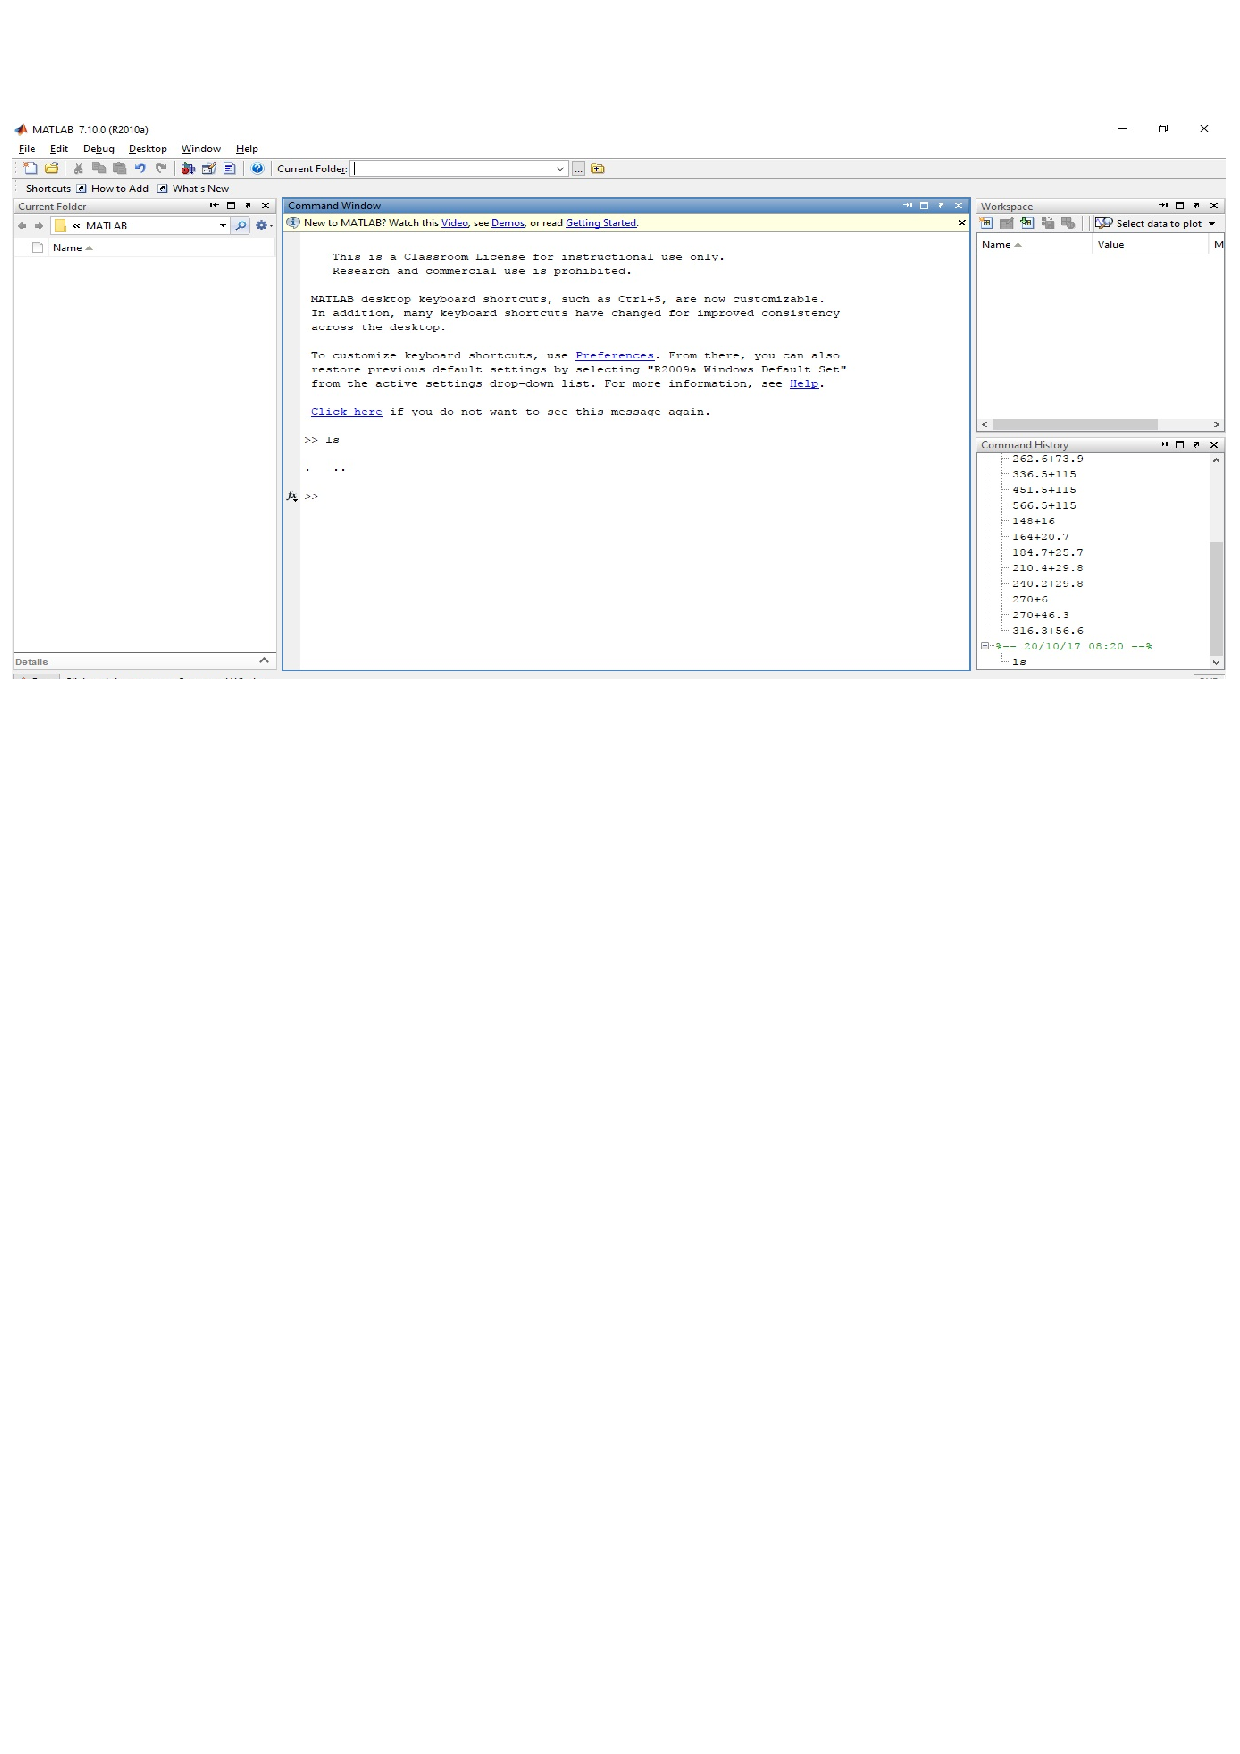
\includegraphics[scale=0.7]{fig1teste.pdf}
    \caption{Abrir o Matlab.}
\end{figure}

\begin{figure}[H]
    \centering
    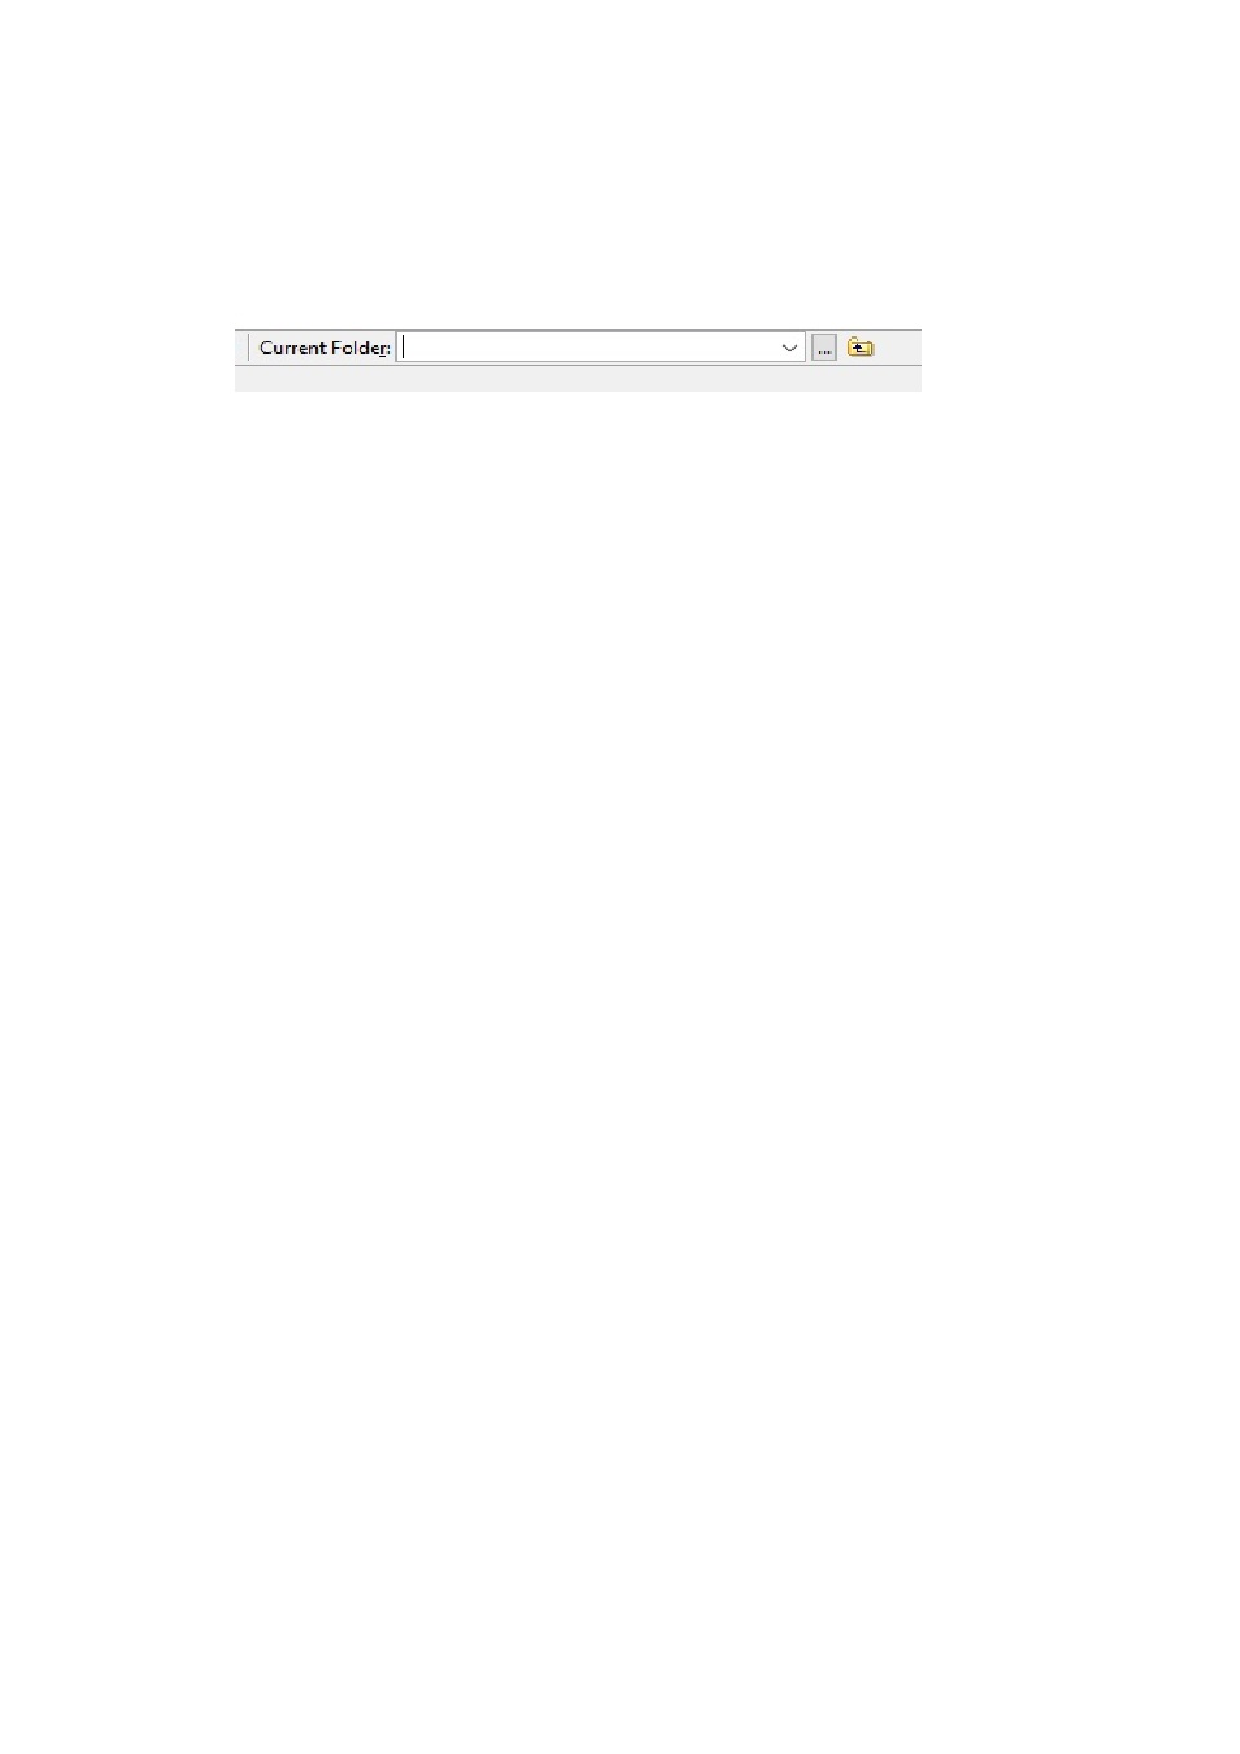
\includegraphics[scale = 0.65]{fig2teste2.pdf}
    \caption{Caixa com três pontos semelhante a reticências ao lado direito de ``Current folder''. Clique nela e selecione o local onde foi salvo o arquivo ``funcsimplex.m''.}
\end{figure}

\begin{figure}[H]
    \centering
    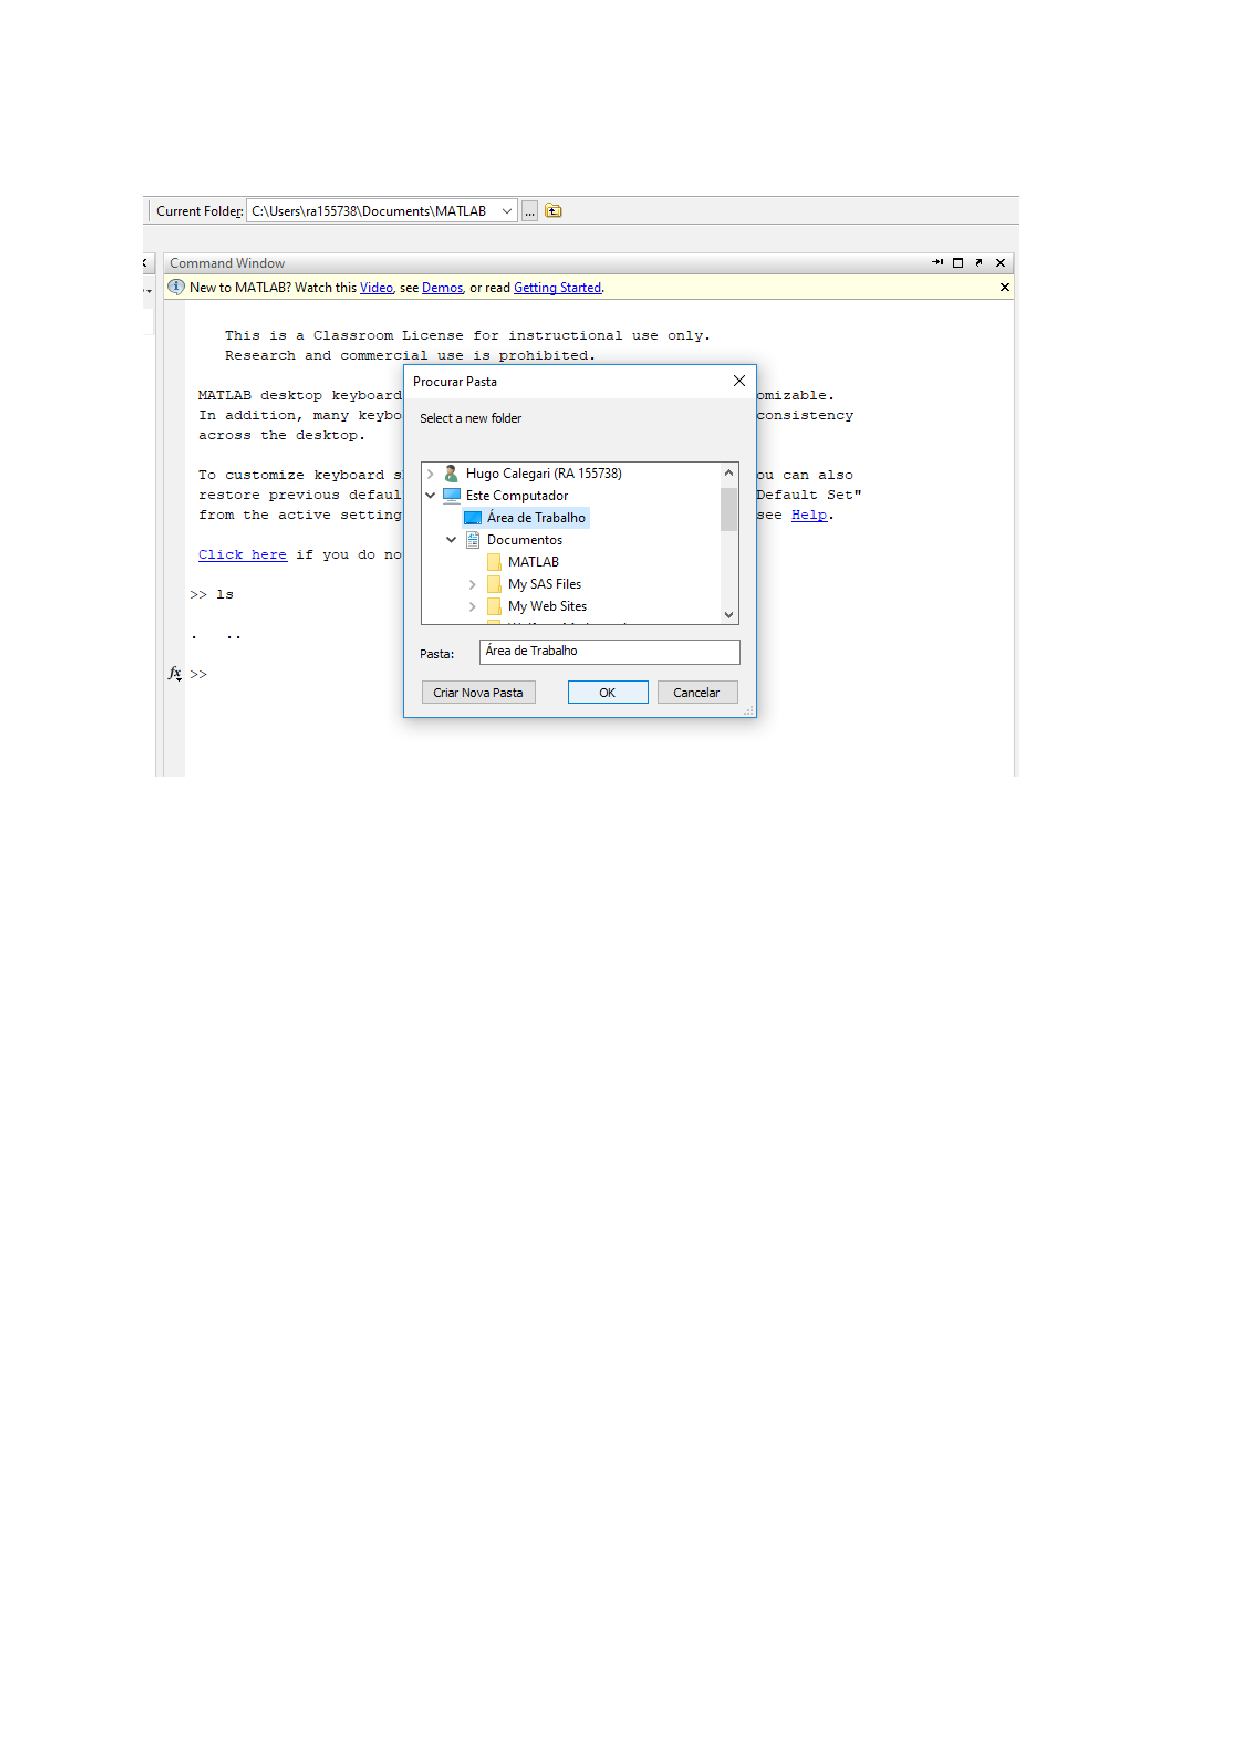
\includegraphics[scale = 0.7]{fig3teste.pdf}
    \caption{Seleção do local onde foi salvo a função do algoritmo primal simplex, definida como ``funcsimplex.m''. Na figura a área de trabalho foi o local onde se salvou a função.}
\end{figure}

\begin{figure}[H]
    \centering
    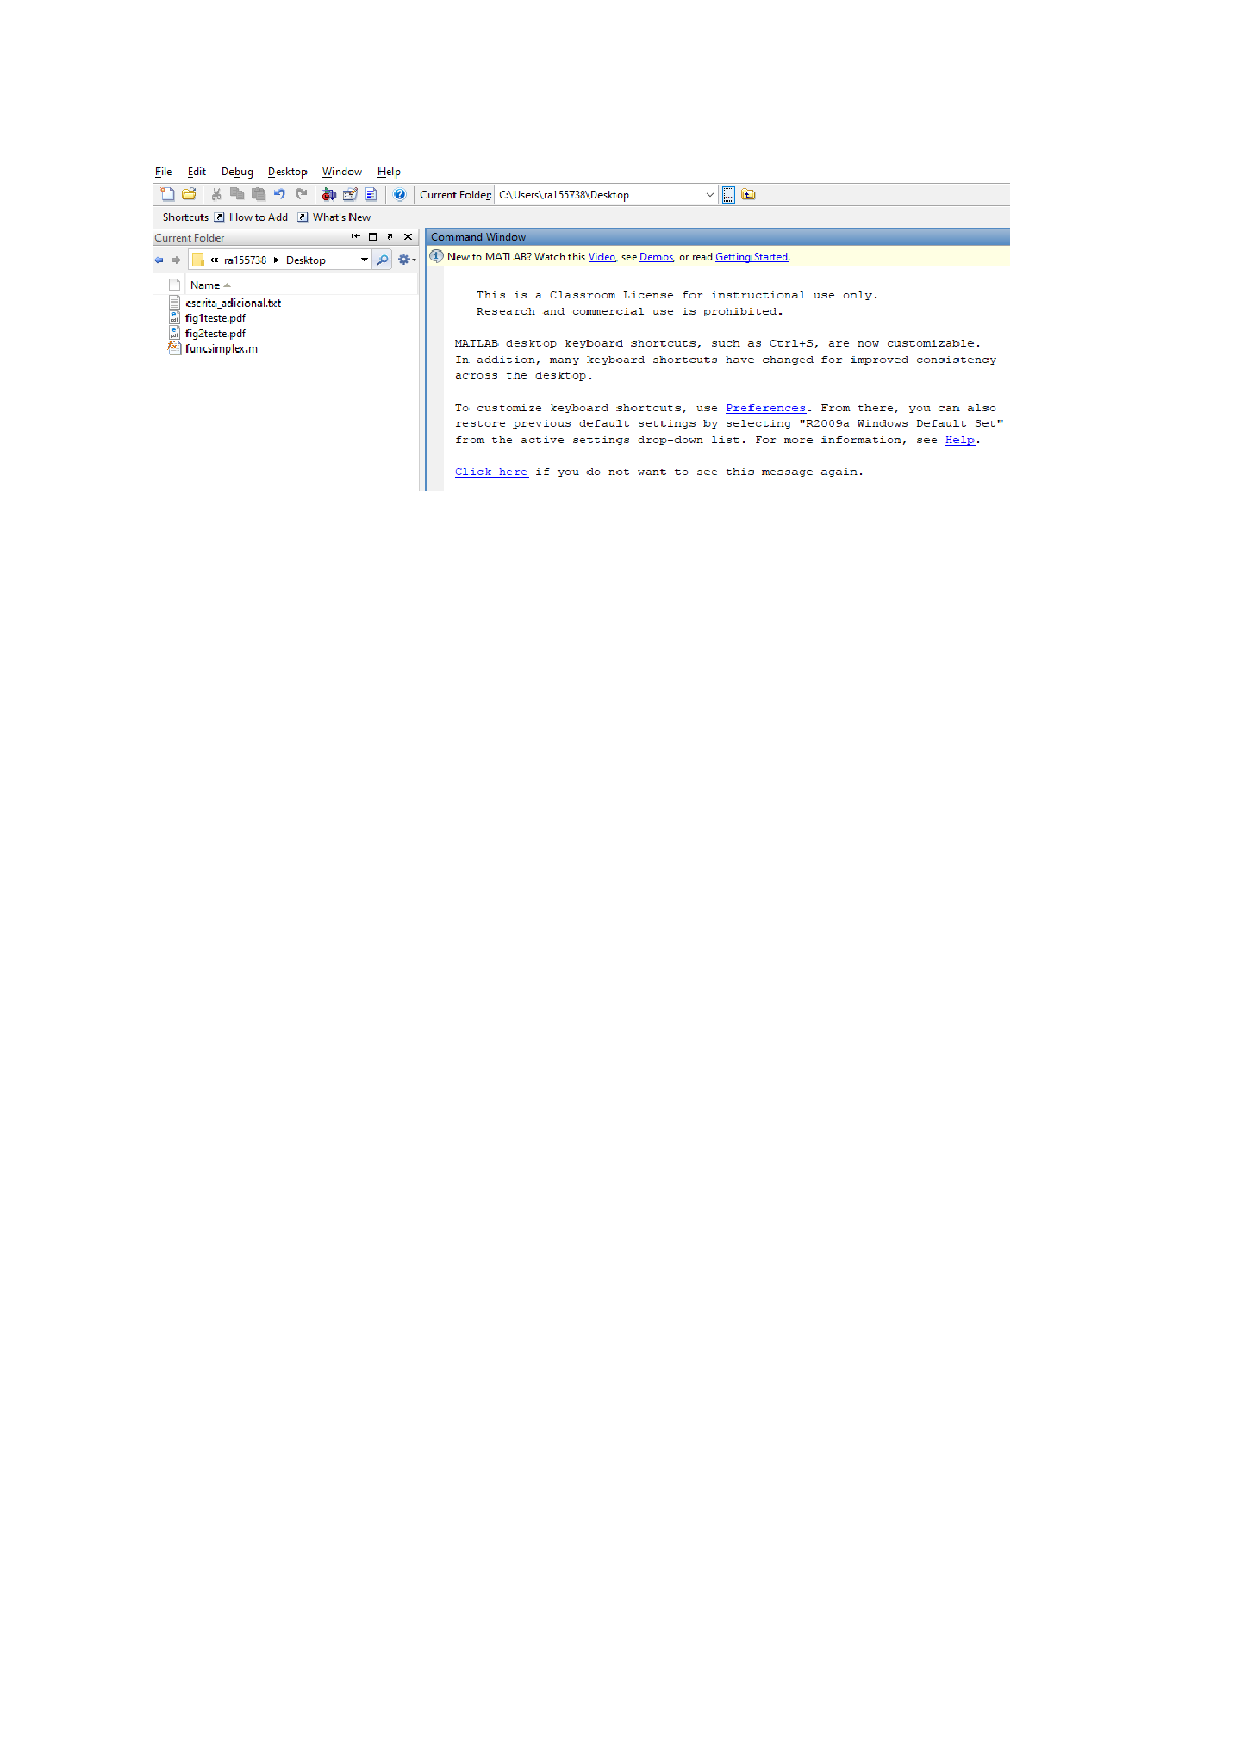
\includegraphics[scale = 0.7]{fig4teste.pdf}
    \caption{Observe que ao lado esquerdo da linha de comando estão listados todos os documentos encontrados na pasta.}
\end{figure}

\begin{figure}[H]
    \centering
    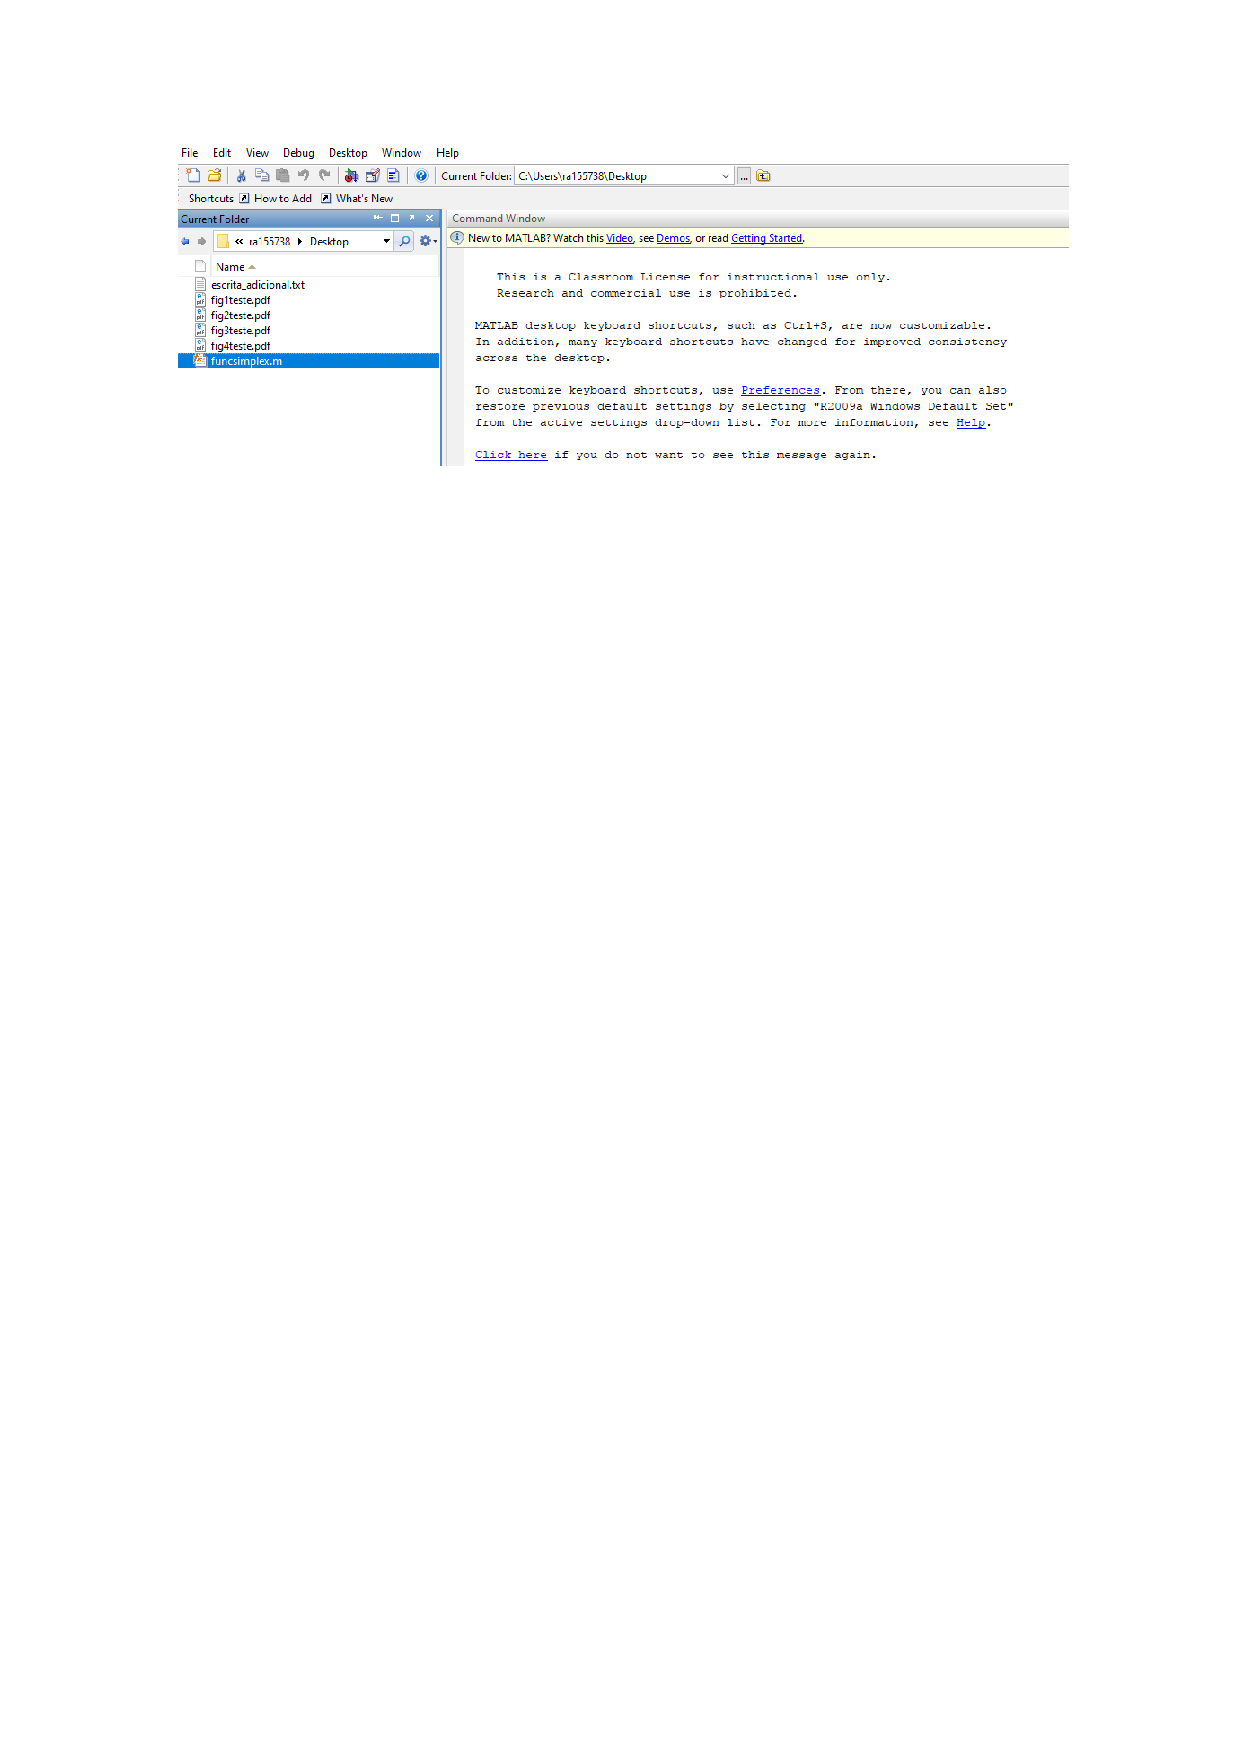
\includegraphics[scale = 0.7]{fig5teste.pdf}
    \caption{Ao clicar duas vezes em ``funcsimplex.m'' o algoritmo do método primal simplex será exibido com todos os comentários feitos.}
\end{figure}

\begin{figure}[H]
    \centering
    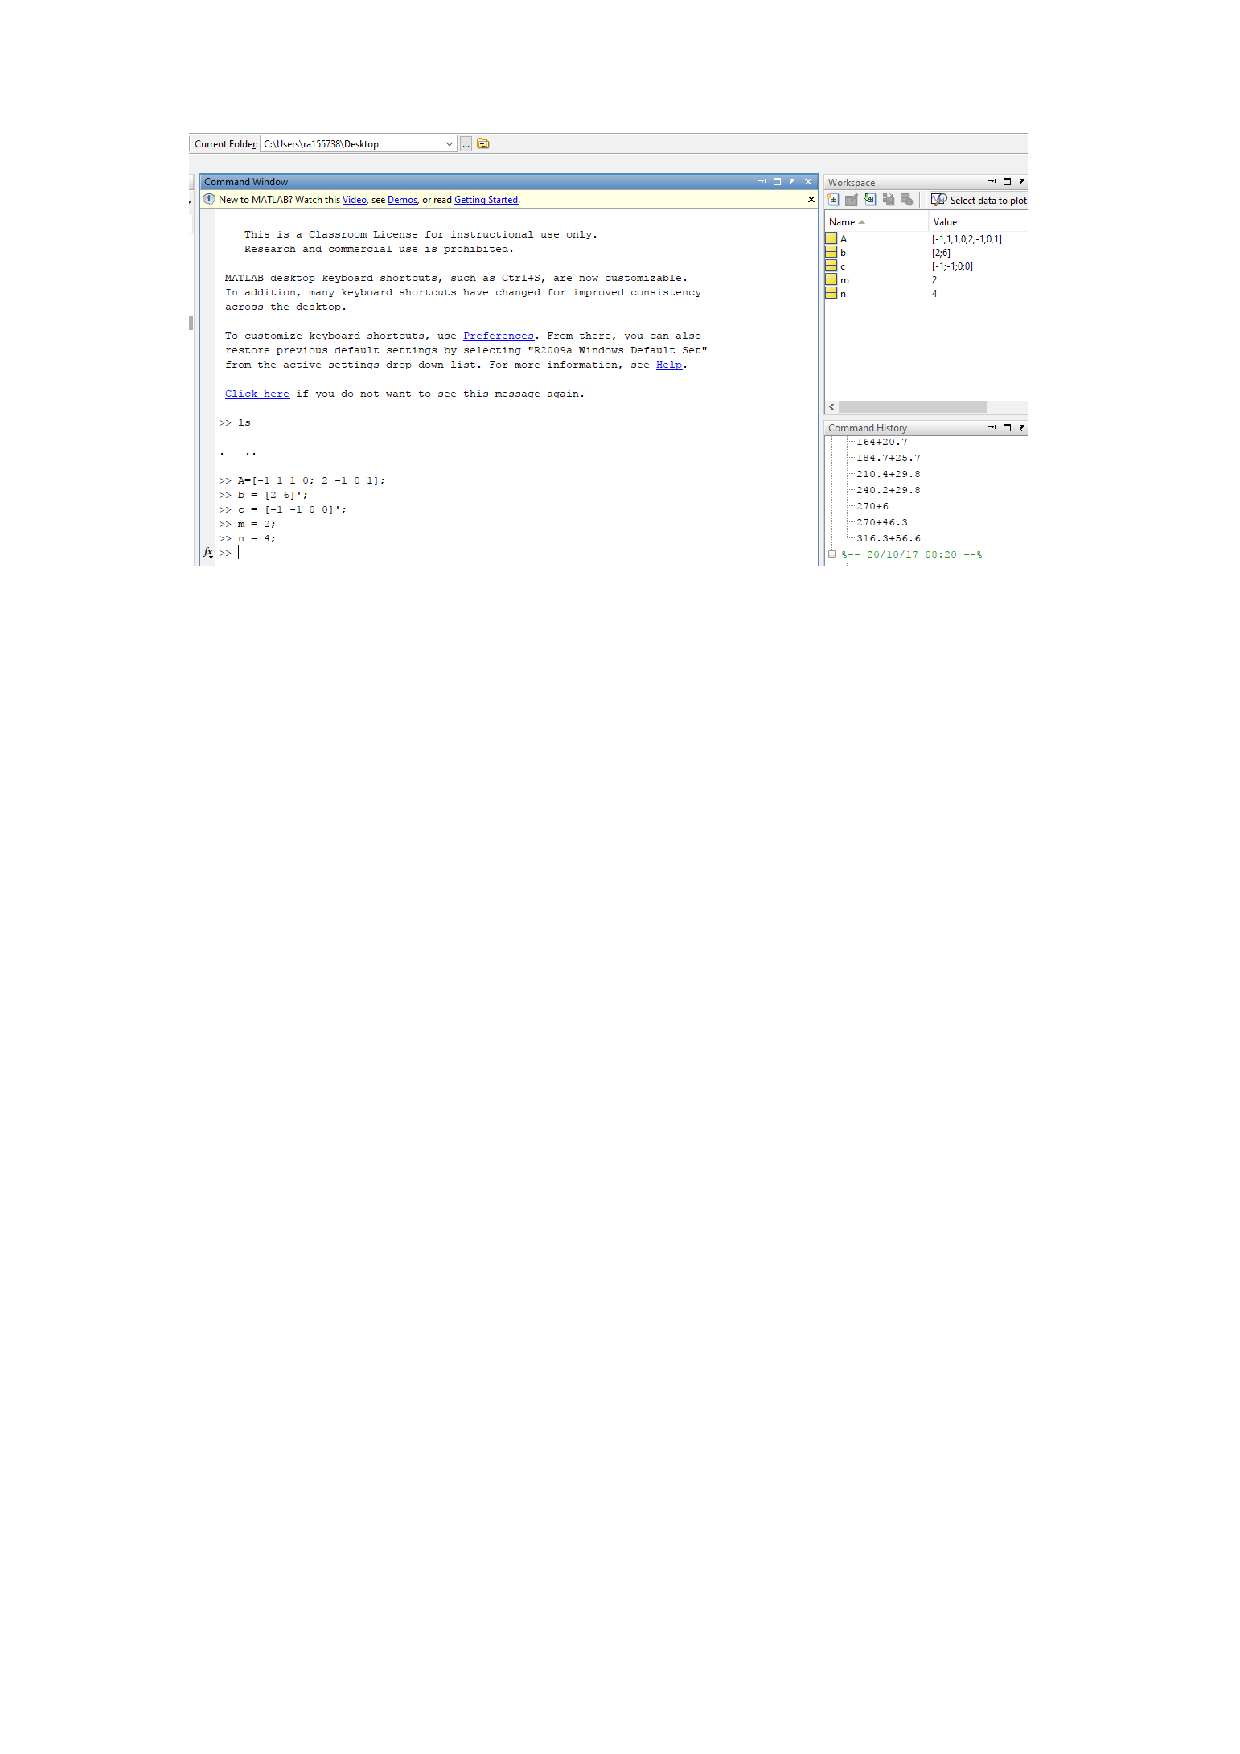
\includegraphics[scale = 0.7]{fig6teste.pdf}
    \caption{Ao digitar a matriz A, os vetores b e c, o número de linhas (m) e colunas (n), note o lado direito da linha de comando (``Workspace''). Neste local estarão todas as variáveis inicializadas.}
\end{figure}


\begin{figure}[H]
    \centering
    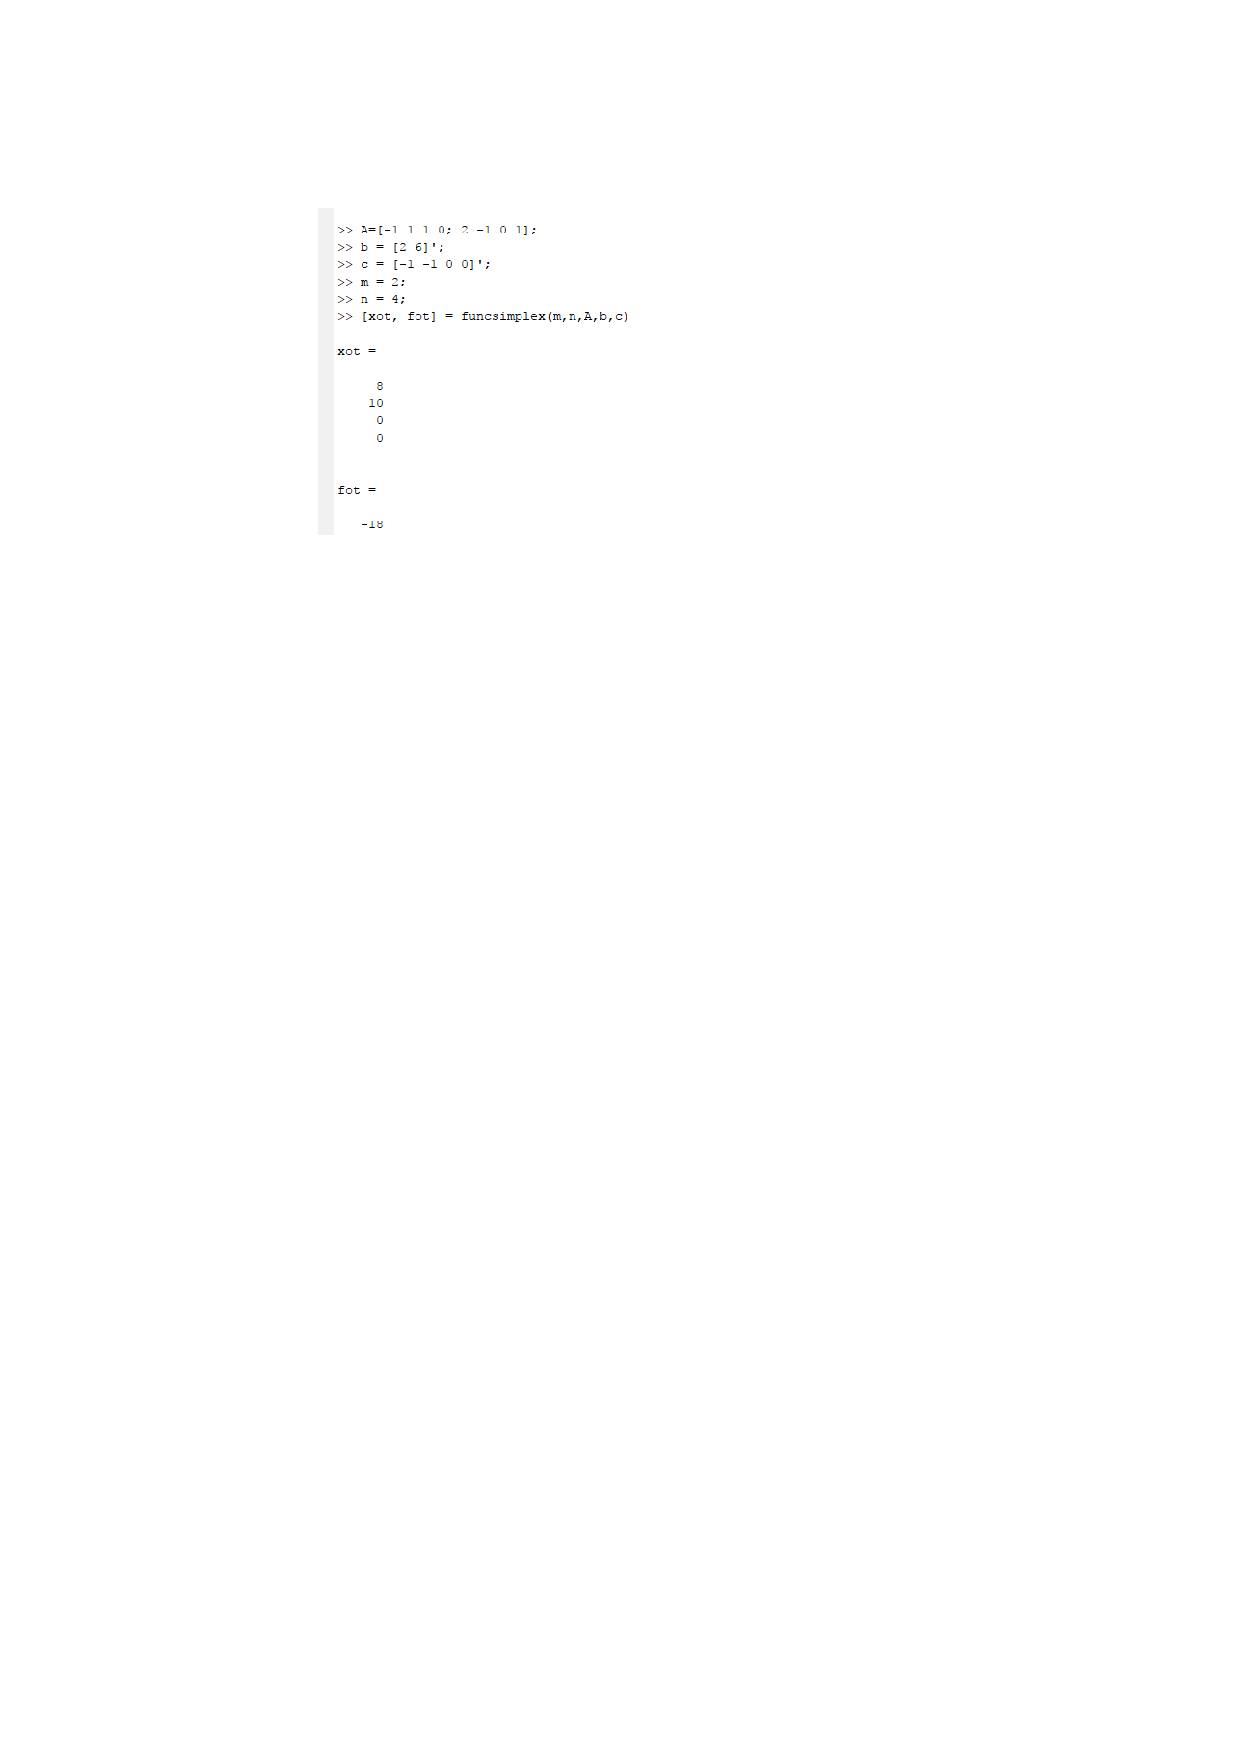
\includegraphics[scale = 0.65]{fig7teste.pdf}
    \caption{Para verificar a solução ótima e a função objetivo mínima associada basta digitar uma linha de comando como a figura mostra.}
\end{figure}

\begin{figure}[H]
    \centering
    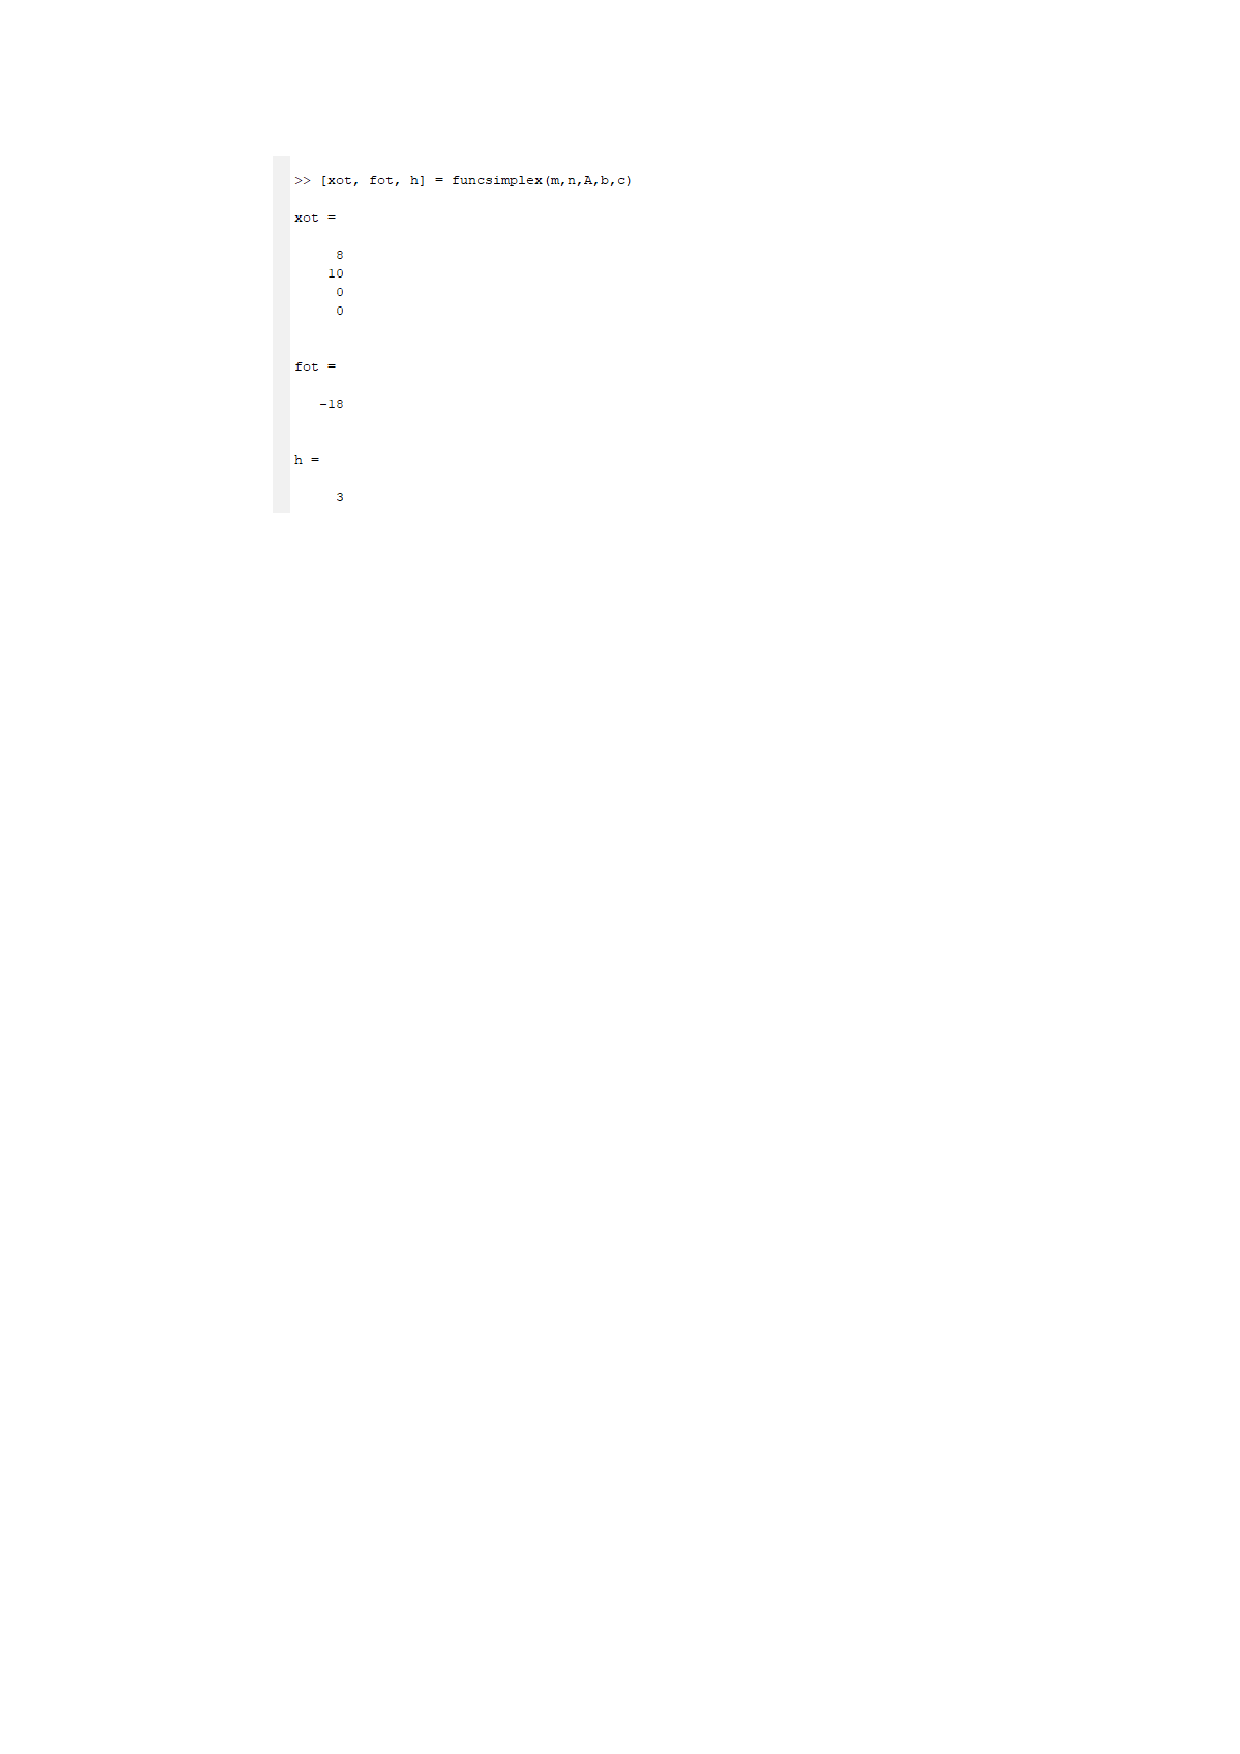
\includegraphics[scale = 0.65]{fig8teste.pdf}
    \caption{Para verificar a solução ótima, a função objetivo mínima associada e o número de iterações realizadas basta digitar uma linha de comando como a figura mostra.}
\end{figure}

\begin{figure}[H]
    \centering
    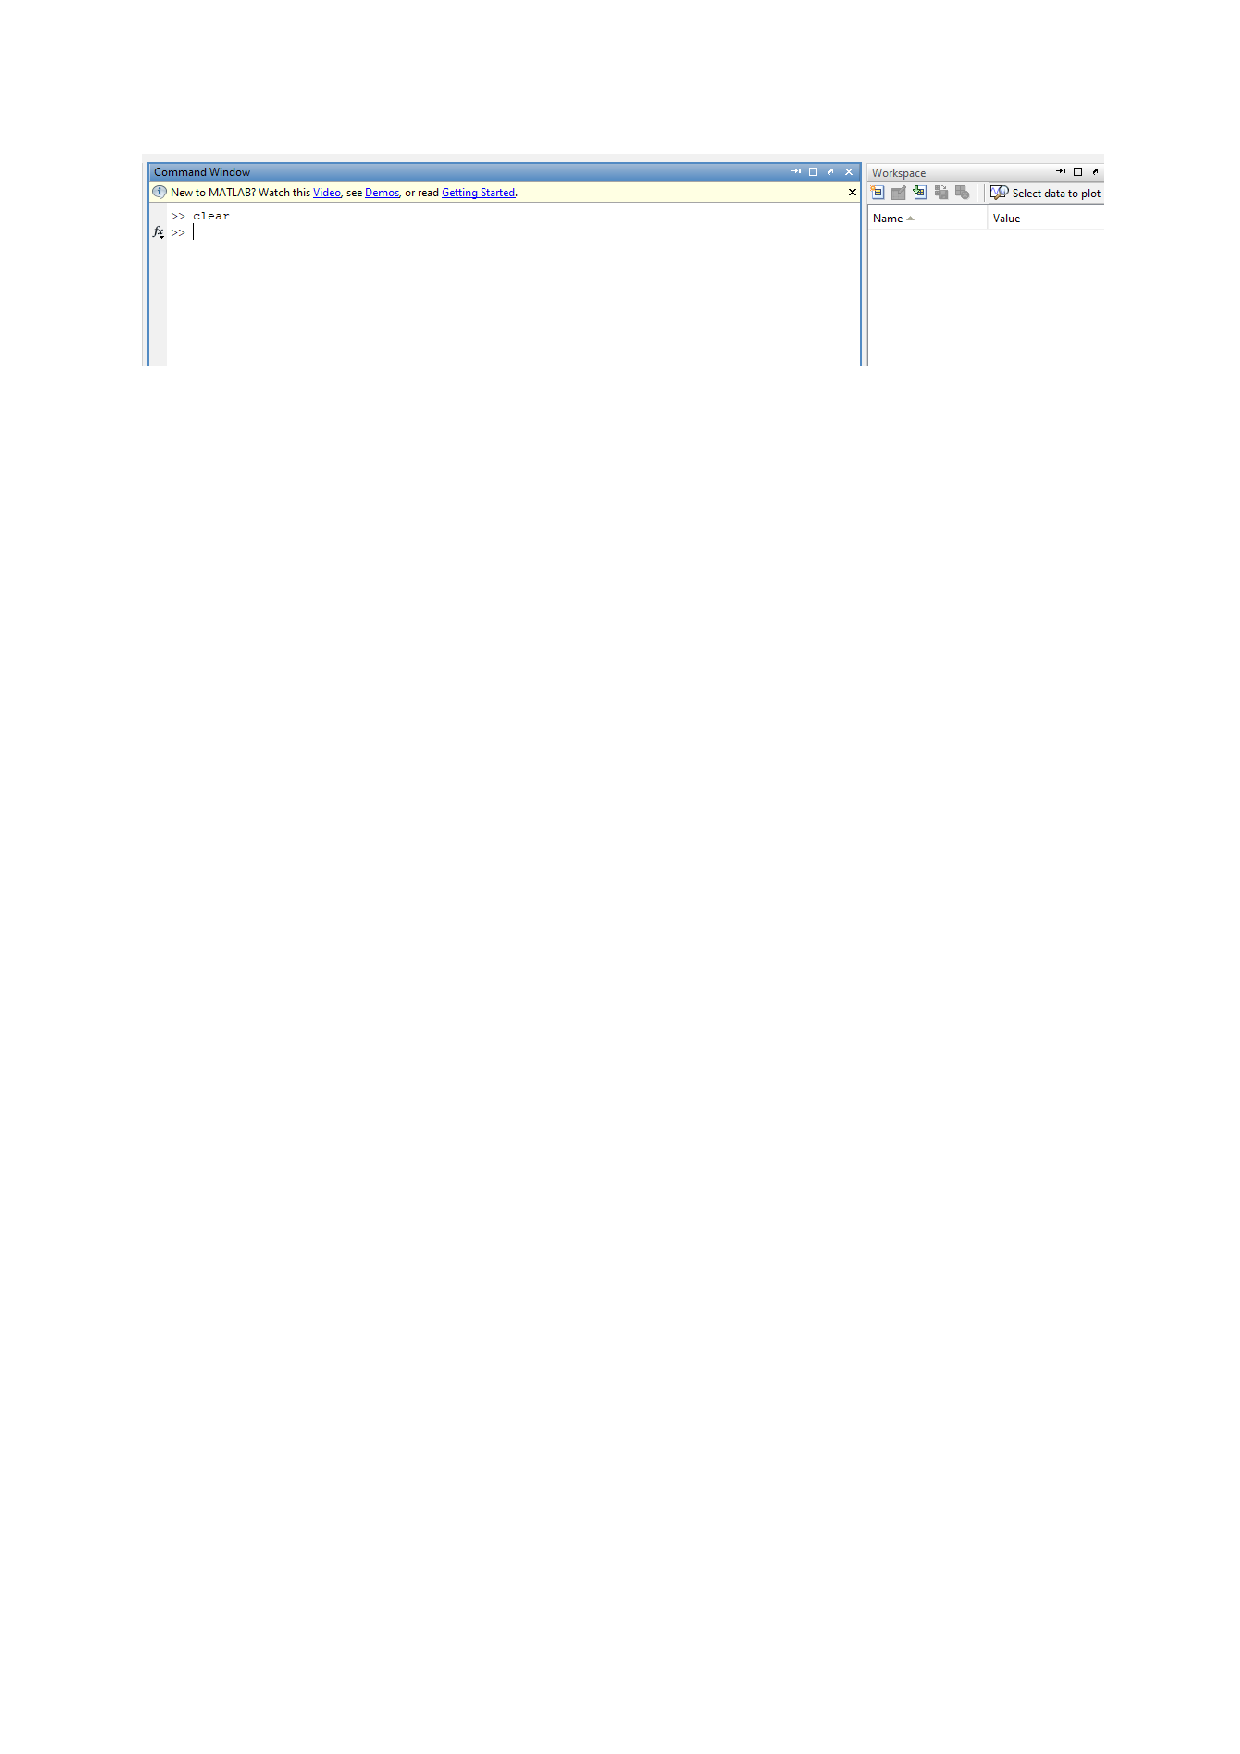
\includegraphics[scale = 0.7]{fig9teste.pdf}
    \caption{Comando ``clear'' para apagar as variáveis que foram utilizadas. Observe que no ``Workspace'' não há nenhuma variável. Caso queira inicializar outros valores de variáveis basta o usuário fornecer os novos valores.}
\end{figure}


\end{document}